% c:\Users\racha\rapport\chapter4\sections\1_useCaseDiagram.tex
La figure~\ref{fig:use_case_diagram} illustre le diagramme de cas d'utilisation pour le Sprint 1, intitulé \textit{Capture et Reconnaissance Texte}. Ce sprint se concentre sur la capture des données à partir d'un moniteur de signes vitaux, leur reconnaissance via une caméra classique et un processus OCR, et la génération d'alertes en fonction des valeurs reconnues.

\begin{figure}[H]
    \centering
    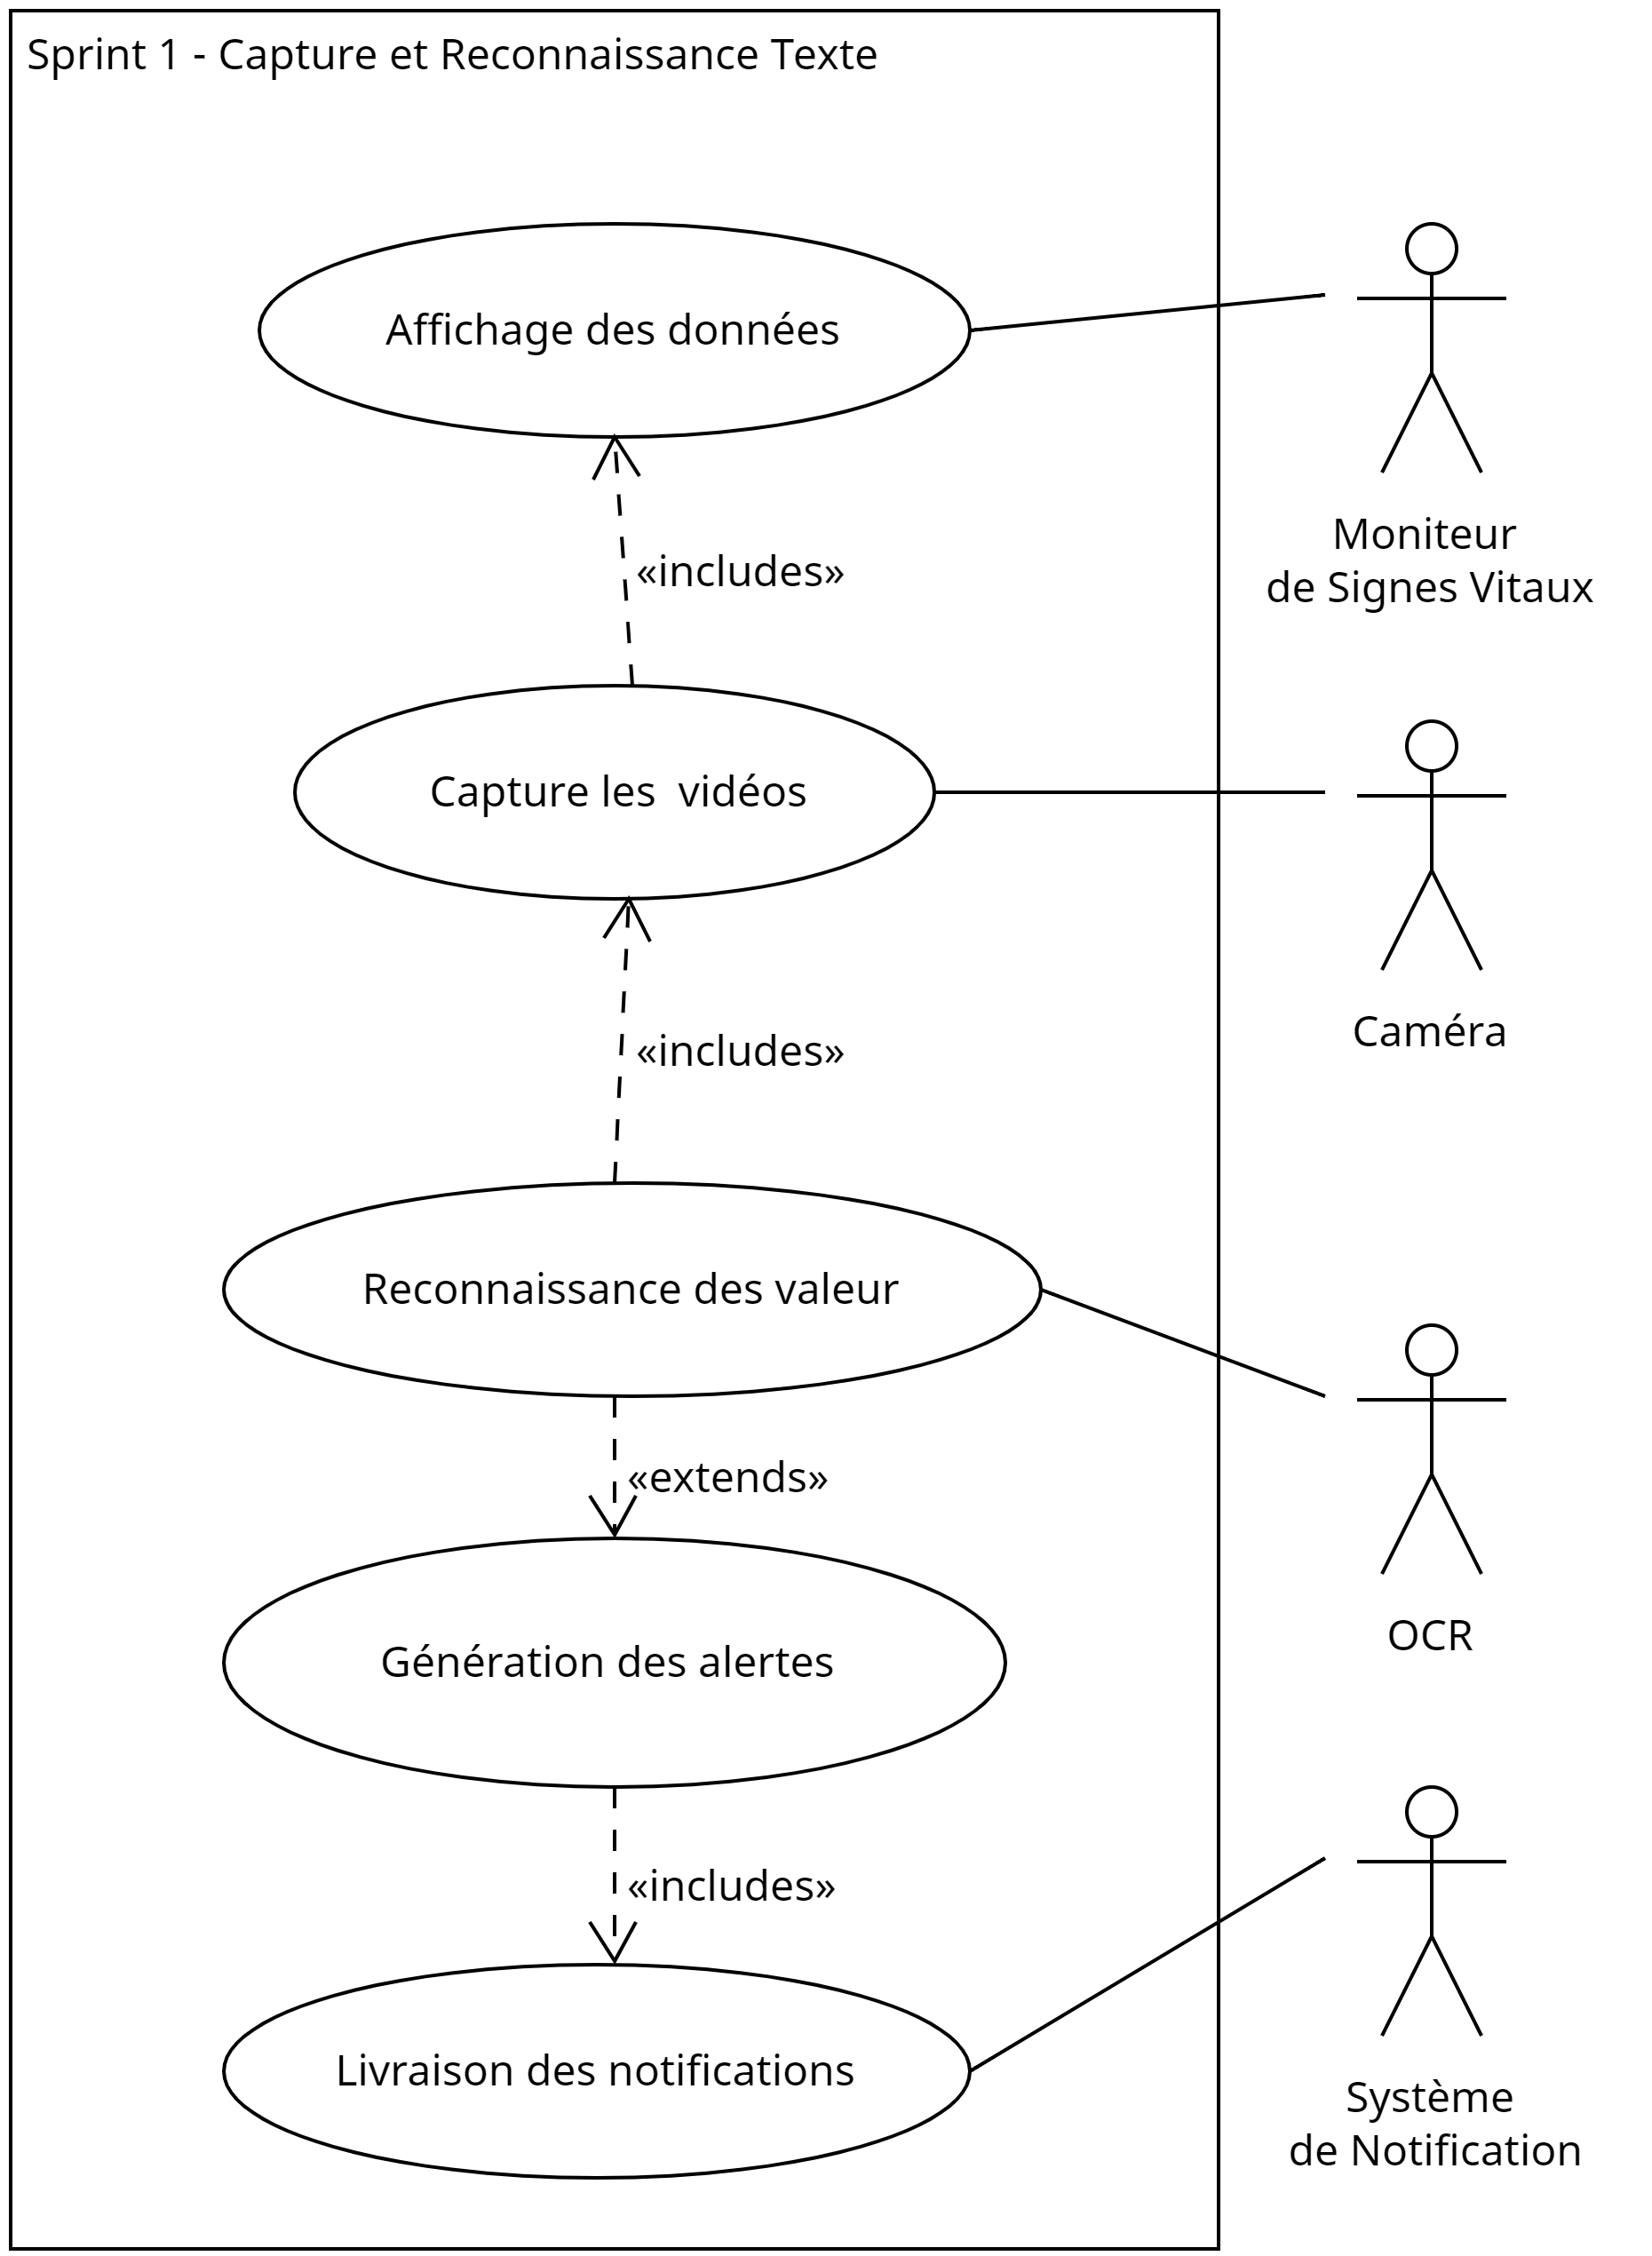
\includegraphics[width=0.8\textwidth]{chapter4/sections/diagrams/Sprint 1 - Capture et Reconnaissance Texte.png}
    \caption{Diagramme de Cas d'Utilisation - Sprint 1}
    \label{fig:use_case_diagram}
\end{figure}



% \subsection{Relations entre Cas d'Utilisation}
% \begin{itemize}
%     \item La reconnaissance des valeurs \textit{«extends»} la génération des alertes.
%     \item L'affichage des données et la livraison des notifications sont \textit{«includes»} dans le processus global.
% \end{itemize}
